
\section{General notes}

\subsection{Running the codes - general rules}
The various program executables are to be run in command mode in the Linux/Unix environment. Each command contains the name of the executable file followed by various options. The options are recognized by being preceded by two minus symbols \verb"--". The program options can be of two kinds: pairs specifying the option followed by the value of the option, of the form [--option-name  value], or flags. The values can be numbers or strings (arrays of characters). The flags are (boolean) switches signaling that a certain action must occur and do not take any value after them. The general syntax to run a program is:
\begin{verbatim} 
    program_name [--option1 val1] [--option2 val2] [...] [--flag1] [...] 
\end{verbatim}
Running \verb"program_name --help" sends a manual page to the screen listing the available flags and options with explanations. 

The order of the options and flags in a command generally does not matter. The specification of certain options is essential for the unambiguous definition of a run, while others are specified only as needed. If any one of the essential options is absent from the command line, the program will warn the user of the missing option and abort.  Additionally, if an unrecognized option or flag is provided, such as a misspelling, the program will also warn the user and abort.

An alternative way to present options to a program is through an options file \verb"program_name.options".  Each line in this text file contains \verb"option-name : value" pairs separated by a colon. Flags are specified by themselves on separate lines. Note that the command line options take precedence over options supplied  in an \verb".options" file, thus a base options file can be constructed and deviations from the baseline can be specified using command-line inputs. Examples of such \verb".options" files are provided in the \verb"samples" directory.

The output of the code is typically saved in text files that are column based. The file names are fixed (hard-coded) and, hopefully, suggestive of their content. All output is saved in the directory from which the run command is given, thus it is often convenient to create a working directory containing all relevant inputs, and run the executables from there. Unless otherwise specified, signal amplitudes are relative to a reference unit amplitude at 1 km. In all cases pressures scaled by the square root of density, $\rho^{-\frac{1}{2}}p$, are written to files rather than the pressure itself. 

\subsection{Atmospheric specifications}
\label{sec: AtmoSpecs}
Necessary input to all propagation codes in this package is the specification of the state of the atmosphere through which propagation is to be modelled. To provide portability and maximum flexibility to the user the state of the atmosphere is input in column-based text files to be provided by the user. Each such file specifies a stratified atmosphere and contains columns such as pressure, density, temperature and the three wind components u, v and w as a function of altitude. The files are self-describing using a formatted header that associates the column with a tag string and an indication of units.  Scalar quantities may also be specified in the header.  Formatted lines and normal (i.e. ignorable) comments may both be used in the header as needed; normal comments are preceded by the \verb"#" character, while formatted lines are preceded with \verb"#%".  Text tags are used to indicate to the modules which columns represent which types of quantities, and are expected to match the following convention:

\begin{minipage}{\linewidth}
\begin{verbatim}
    Z   - altitude above MSL
    U   - West-to-East wind speed
    V   - South-to-North wind speed
    T   - temperature
    RHO - density
    P   - ambient pressure
    C0  - static sound speed (optional, will be calculated if not provided)
    Z0  - ground elevation (scalar, optional)
\end{verbatim}
\end{minipage}

\noindent Any unrecognized tags will be ignored. Tags beginning and ending with underscores (for example \verb"_ALPHA_") should not be used, as this convention is used for internally-calculated quantities and may cause conflicts. Scalar quantities are indicated using column number \verb"0" and are in the format \verb"0, <tag>, <units>, <value>", while vector quantities use the format \verb"<column>, <tag>, <units>" with values provided in the columns.  Altitude, as the independent quantity, must be provided in column number \verb"1".  An example of a formatted header with units and a scalar quantity demonstrates this:

\begin{minipage}{\linewidth}
\begin{verbatim}
#% 0, Z0, m, 45.0
#% 1, Z, km
#% 2, U, m/s
#% 3, V, m/s
#% 4, W, m/s
#% 5, T, degK
#% 6, RHO, g/cm3
#% 7, P, mbar
\end{verbatim}
\end{minipage}

\noindent In this example, the static sound speed \verb"C0" will be calculated internally from the pressure and density.

Quantities may be provided in any supported units and will be converted internally as needed.  Additional units may be added by the user as needed by following the directions given in the comment header in \verb"src/common/units.h".  Supported units as of this release may be indicated by any of the following codes, which are case-insensitive:

\begin{minipage}{\linewidth}
\begin{verbatim}
    temperature: K, DEGK, DEG K, DEGREES K
                 C, DEGC, DEG C, DEGREES C
                 F, DEGF, DEG F, DEGREES F
    distance:    M, METERS
                 KM, KILOMETERS
    speed:       M/S, MPS, MPERS, M PER S, METERS PER SECOND
                 KM/S, KMPS, KMPERS, KM PER S, KILOMETERS PER SECOND
    pressure:    PA, PASCAL, PASCALS
                 MBAR, MILLIBAR, MILLIBARS
    density:     KG/M3, KGPM3, KILOGRAMS PER CUBIC METER
                 G/CM3, GPCM3, GRAMS PER CUBIC CENTIMETER
    direction:   DEGREES CLOCKWISE FROM NORTH, DEG CW FROM N, AZIMUTH
                 DEGREES COUNTERCLOCKWISE FROM EAST, DEG CCW FROM E
    angle:       DEG, DEGREES
                 RAD, RADIANS
\end{verbatim}
\end{minipage}

\begin{figure}
\begin{center}
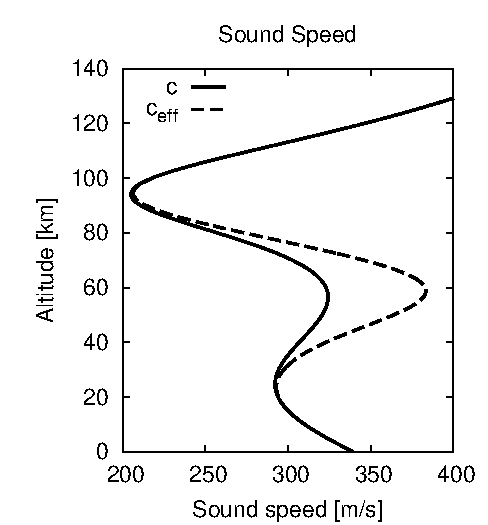
\includegraphics[scale=0.62]{figs/model_atmos_c}
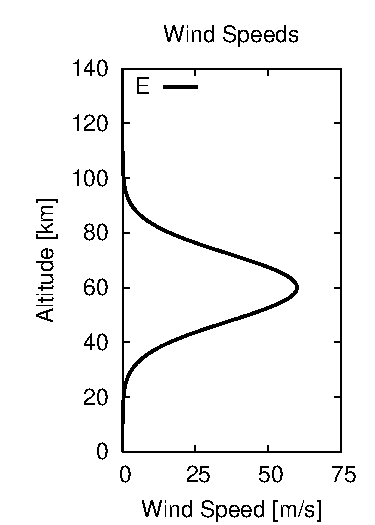
\includegraphics[scale=0.62]{figs/model_atmos_winds_u}
\end{center}
\caption{The NCPA model atmosphere, the ``toy'' model. The figure on the left shows sound speeds: the solid curve is the adiabatic sound speed and the dashed curve is the effective sound speed profile in the azimuth direction of 90 degrees (clockwise from North). The figure on the right shows the model zonal wind speed. The meridional wind speed is taken to be zero. The figures are taken from \cite{waxler2015stratospheric}.}
\label{fig:canonic_sound_speeds}
\end{figure}

An example of an atmospheric profile file with the above structure is provided in the \verb"samples" directory in file \verb"NCPA_canonical_profile_trimmed.dat". Most tutorial examples included in this or the on-line help are based on this profile. The corresponding sound speed, effective sound speed for azimuth of $90\degree$ and wind speed are illustrated in Figure \ref{fig:canonic_sound_speeds}.  Alternately, a separate file containing only the descriptive header may be specified using the command-line flag \verb"--atmosheaderfile".  If this flag is used, the indicated file will provide the profile metadata and any formatted header in the profile file will be ignored.  An example of this file is provided in the \verb"samples" directory in file \verb"sampleheader.dat" and an example of the proper usage is given as the first sample command in the {\bf WMod} package.

To model propagation through a stratified medium only a single specification file is required. Range dependent profiles for the \verb"ePape" module are specified by providing a summary file that associates a range (in km) with a 1-D atmospheric file in the above format, for example:

\begin{minipage}{\linewidth}
\begin{verbatim}
0.0   profiles/profile0000.dat
89.0  profiles/profile0089.dat
179.0 profiles/profile0179.dat
269.0 profiles/profile0269.dat
359.0 profiles/profile0359.dat
\end{verbatim}
\end{minipage}

\noindent The resulting 2-d specification is piecewise stratified with transitions at the midpoints between the indicated ranges. Additional range-dependent formats are under development.